\documentclass[aspectratio=169]{beamer}

\mode<presentation>
{
  \usetheme{default}
  \usecolortheme{default}
  \usefonttheme{default}
  \setbeamertemplate{navigation symbols}{}
  \setbeamertemplate{caption}[numbered]
  \setbeamertemplate{footline}[frame number]  % or "page number"
  \setbeamercolor{frametitle}{fg=white}
  \setbeamercolor{footline}{fg=black}
} 

\usepackage[english]{babel}
\usepackage[utf8x]{inputenc}
\usepackage{tikz}
\usepackage{courier}
\usepackage{array}
\usepackage{bold-extra}
\usepackage{minted}
\usepackage[thicklines]{cancel}

\xdefinecolor{dianablue}{rgb}{0.18,0.24,0.31}
\xdefinecolor{darkblue}{rgb}{0.1,0.1,0.7}
\xdefinecolor{darkgreen}{rgb}{0,0.5,0}
\xdefinecolor{darkgrey}{rgb}{0.35,0.35,0.35}
\xdefinecolor{darkorange}{rgb}{0.8,0.5,0}
\xdefinecolor{darkred}{rgb}{0.7,0,0}
\definecolor{darkgreen}{rgb}{0,0.6,0}
\definecolor{mauve}{rgb}{0.58,0,0.82}

\title[2017-12-08-uproot-update]{\Huge uproot update}
\author{Jim Pivarski}
\institute{Princeton University -- DIANA-HEP}
\date{December 12, 2017}

\begin{document}

\logo{\pgfputat{\pgfxy(0.11, 7.4)}{\pgfbox[right,base]{\tikz{\filldraw[fill=dianablue, draw=none] (0 cm, 0 cm) rectangle (50 cm, 1 cm);}\mbox{\hspace{-8 cm}
\includegraphics[height=1 cm]{princeton-logo-long.png}
\includegraphics[height=1 cm]{diana-hep-logo-long.png}}}}}

\begin{frame}
  \titlepage
\end{frame}

\logo{\pgfputat{\pgfxy(0.11, 7.4)}{\pgfbox[right,base]{\tikz{\filldraw[fill=dianablue, draw=none] (0 cm, 0 cm) rectangle (50 cm, 1 cm);}\mbox{\hspace{-8 cm}
\includegraphics[height=1 cm]{princeton-logo.png}
\includegraphics[height=1 cm]{diana-hep-logo.png}}}}}

% Uncomment these lines for an automatically generated outline.
%\begin{frame}{Outline}
%  \tableofcontents
%\end{frame}

% START START START START START START START START START START START START START

\begin{frame}{(Everybody take a look at the ZEBRA manual!)}
\vspace{0.6 cm}
\begin{center}
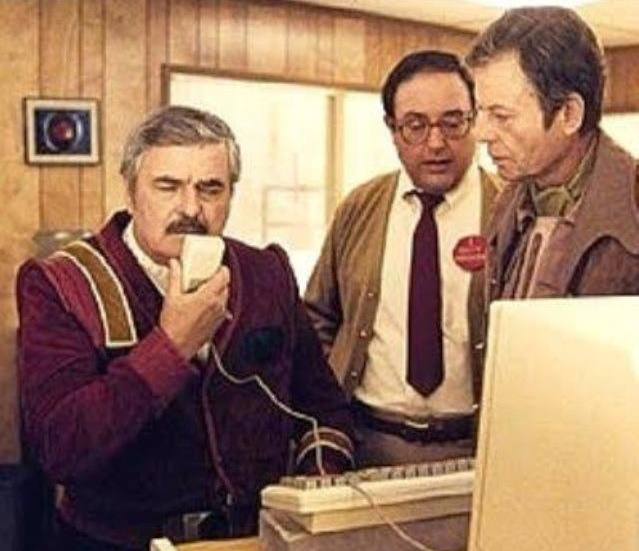
\includegraphics[height=6 cm]{scotty.jpg}

\LARGE ``Hello, computer?''
\end{center}
\end{frame}

\begin{frame}{``Data bank'' management systems}
\vspace{0.25 cm}
\begin{center}
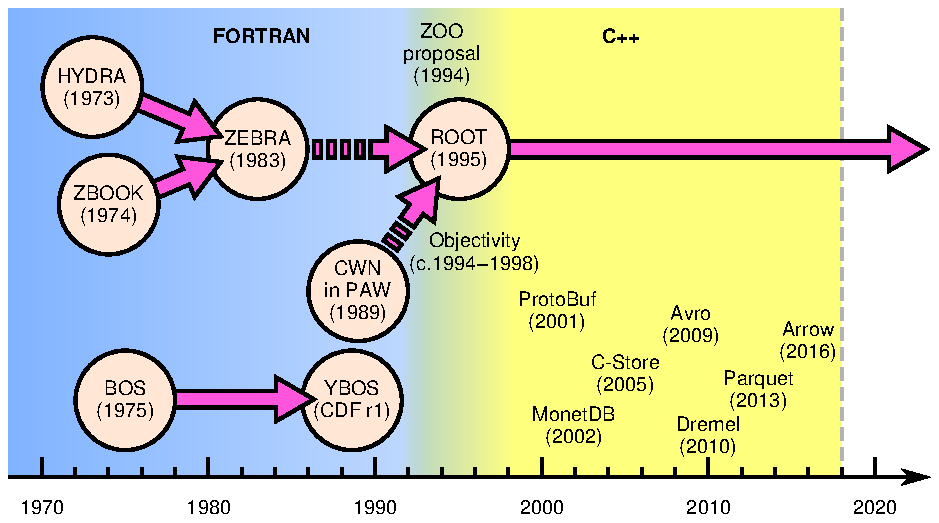
\includegraphics[width=0.95\linewidth]{history.pdf}
\end{center}
\end{frame}

\begin{frame}{File formats {\it and specifications}}
\vspace{0.5 cm}
\begin{columns}
\column{1.1\linewidth}
\renewcommand{\arraystretch}{1.5}
\begin{tabular}{l c c c}
& inception & specification & implementations \\\hline

FITS & 1981 & \href{https://fits.gsfc.nasa.gov/standard30/fits_standard30aa.pdf}{\textcolor{blue}{\tiny https://fits.gsfc.nasa.gov/standard30/fits\_standard30aa.pdf}} & 38 \\

netCDF,HDF4/5 & 1992 & \href{https://support.hdfgroup.org/HDF5/doc/H5.format.html}{\textcolor{blue}{\tiny https://support.hdfgroup.org/HDF5/doc/H5.format.html}} & 35 \\

ROOT & 1995 & {\tiny some class headers like \href{https://root.cern.ch/doc/master/classTFile.html}{\textcolor{blue}{TFile}} and \href{https://root.cern.ch/doc/master/classTKey.html}{\textcolor{blue}{TKey}}; not enough info to read a file} & 6 \\

Pickle & 1996 & {\tiny {\it implementation} changes: 1$\to$2 \href{http://legacy.python.org/dev/peps/pep-0307/}{\textcolor{blue}{PEP-307}}, 3$\to$4 \href{https://www.python.org/dev/peps/pep-3154/}{\textcolor{blue}{PEP-3154}}; not a real spec} & 4 \\

Protocol buffers & 2001 & \href{https://developers.google.com/protocol-buffers/docs/encoding}{\textcolor{blue}{\tiny https://developers.google.com/protocol-buffers/docs/encoding}} & 20 \\

Thrift & 2007 & {\tiny {\bf UNOFFICIAL:} \href{https://erikvanoosten.github.io/thrift-missing-specification/}{\textcolor{blue}{\tiny https://erikvanoosten.github.io/thrift-missing-specification/}}} & 15 \\

Avro & 2009 & \href{http://avro.apache.org/docs/current/spec.html}{\textcolor{blue}{\tiny http://avro.apache.org/docs/current/spec.html}} & 13 \\

Parquet & 2013 & \href{http://parquet.apache.org/documentation/latest/}{\textcolor{blue}{\tiny http://parquet.apache.org/documentation/latest/}} & 5 \\

Arrow/Feather & 2016 & \href{https://arrow.apache.org/docs/memory_layout.html}{\textcolor{blue}{\tiny https://arrow.apache.org/docs/memory\_layout.html}} & 7 \\
\end{tabular}
\end{columns}
\end{frame}

\begin{frame}
\vspace{1 cm}
\begin{columns}
\column{0.7\linewidth}
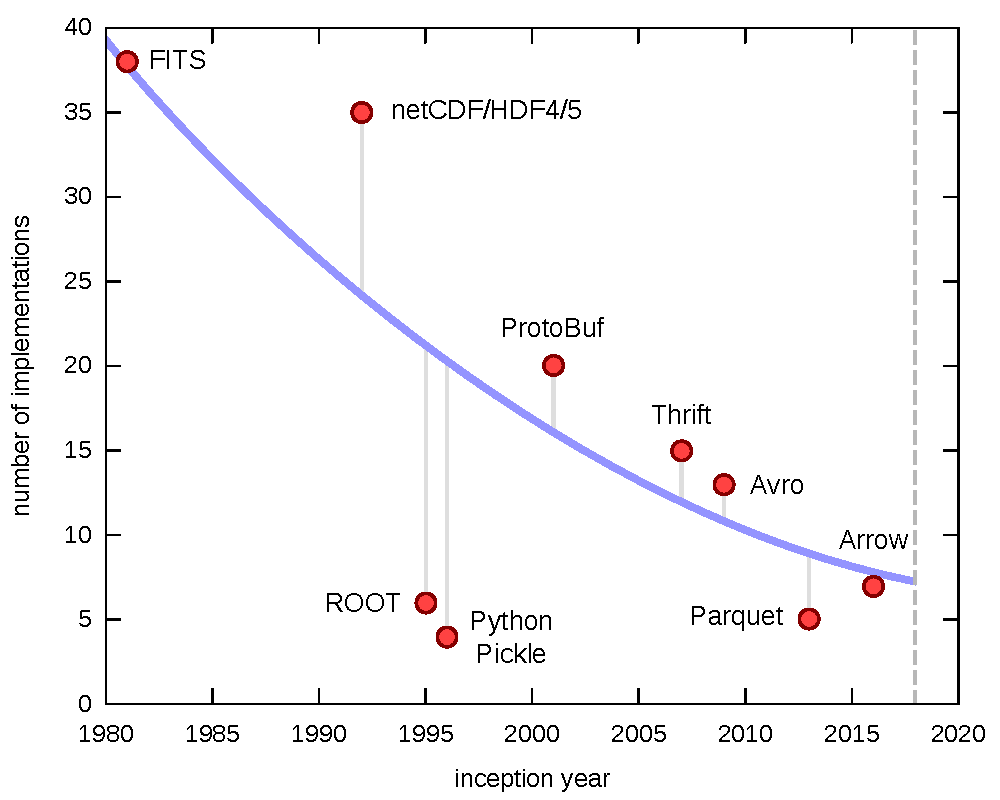
\includegraphics[width=\linewidth]{specs.pdf}

\column{0.35\linewidth}
\textcolor{darkblue}{\underline{General trend}}

\vspace{0.1 cm}
File formats that are used for many years accumulate implementations, to access the data in different ways.

\small

\vspace{0.4 cm}
\uncover<2->{\textcolor{darkblue}{Outlier:} netCDF/HDF4/5 may be too broad to call one format.}

\vspace{0.2 cm}
\uncover<3->{\textcolor{darkblue}{Outlier:} Python Pickle is only reimplemented when the language is reimplemented.}

\vspace{0.2 cm}
\uncover<4->{\textcolor{darkblue}{Outlier:} the ROOT format is defined by its implementation, not a specification, making it hard to reimplement.}

\end{columns}
\end{frame}

\begin{frame}{ROOT I/O implementations}
\vspace{0.25 cm}
\begin{columns}
\column{1.1\linewidth}
\renewcommand{\arraystretch}{1.6}
\begin{tabular}{p{2 cm} c p{4.7 cm} p{5.25 cm}}
\centering ROOT & C++ & ROOT itself. & The ROOT team \\
\centering JsRoot & Javascript & For interacting with ROOT in web browsers or standalone. & Bertrand Bellenot, Sergey Linev (within the ROOT team) \\
\centering root4j/ spark-root & Java/Scala & For Spark and other Big Data projects that run on Java. & Started by Tony Johnson in 2001, updated by Viktor Khristenko \\
\centering inlib/exlib & C++ & Intended as an alternative, embedded in GEANT-4. & Guy Barrand \\
\centering rootio & Go & go-hep ecosystem in Go. & Sebastien Binet \\
\centering \only<1>{\textcolor{black}{uproot}}\only<2>{\textcolor{blue}{uproot}} & \only<1>{\textcolor{black}{Python}}\only<2>{\textcolor{blue}{Python}} & \only<1>{\textcolor{black}{For quickly getting ROOT data into Numpy and Pandas for machine learning.}}\only<2>{\textcolor{blue}{For quickly getting ROOT data into Numpy and Pandas for machine learning.}} & \only<1>{\textcolor{black}{Jim Pivarski (me)}}\only<2>{\textcolor{blue}{Jim Pivarski (me)}} \\
& Rust? & & \\
\end{tabular}
\end{columns}
\end{frame}

\begin{frame}{Motivations for uproot}
\vspace{0.25 cm}
\begin{center}
\only<1>{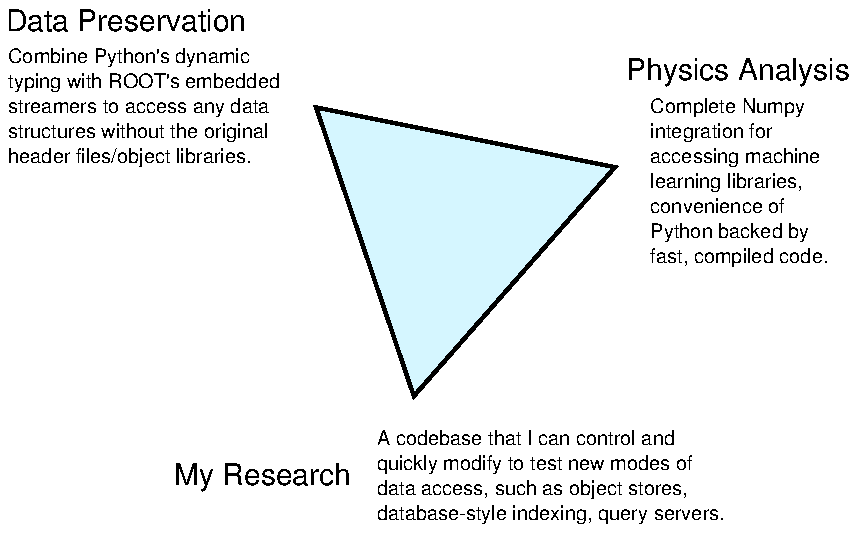
\includegraphics[width=0.85\linewidth]{motivations.pdf}}
\only<2>{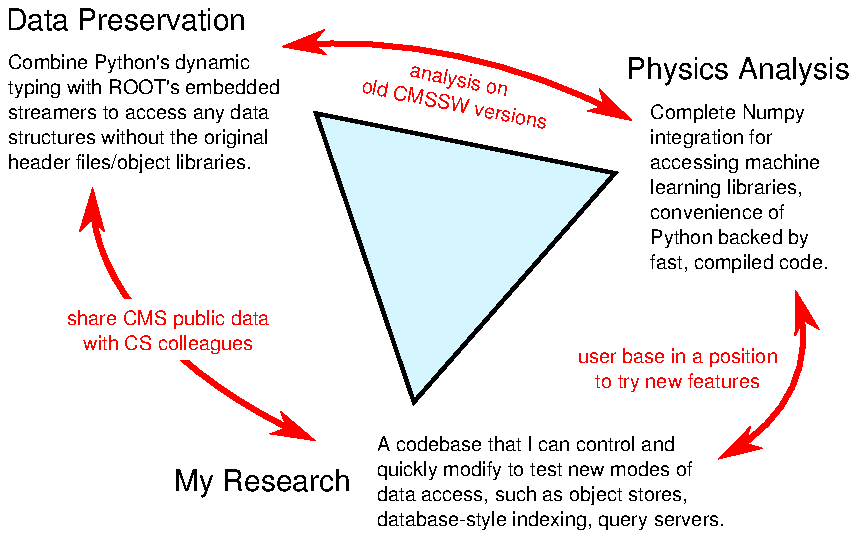
\includegraphics[width=0.85\linewidth]{motivations-2.pdf}}
\end{center}
\end{frame}


\end{document}
